
\lstset{basicstyle=\footnotesize\ttfamily,
        emphstyle=\bfseries,
        columns=fixed,
        numbers=none,
        moredelim=*[l][\textit]{//},
        moredelim=*[l][\bfseries]{\#},
        literate={...}{\dots}3
} 
\section{Criticality-Aware Task Scheduler (CATS)}
\label{sec.scheduling.cats}
The Criticality-Aware Task Scheduling generally applies to task-based programming models supporting task dependencies, but for simplicity we explain it in the context of the OmpSs programming model.
CATS uses bottom-level longest-path priorities and consists of three steps:
%\begin{itemize}

\textbf{Task prioritization}: when a task is created and added to the TDG, it is assigned a priority and the priority of the rest of tasks in the graph is updated accordingly.
 %Since the task graph is generated at runtime, there is no way to statically compute the priority that will be given to a task. 

\textbf{Task submission}: when a task becomes \textit{ready}, i.e., all its predecessors finished their execution, it is submitted to a \textit{ready queue}. At this point, the algorithm decides whether the task is considered \textit{critical} or \textit{non critical}. The task is then inserted in the corresponding ready queue: tasks in the \textit{critical ready queue} will be executed by fast cores, and tasks in the \textit{non-critical ready queue} will be executed by slow cores.

\textbf{Task-to-core assignment}: when a core becomes idle, it retrieves a task from one of the two ready queues to execute. 
The different policies and scenarios of this step are detailed in Section~\ref{sec.cats.assignment}.

%If the queue is empty, it might try to steal from the other queue according on the work stealing policy. %Currently, we support two work stealing mechanisms: \textit{simple} work stealing, i.e., fast cores can steal from slow cores; and \textit{bidirectional} (\textit{2DS}) work stealing, i.e., both types can steal from the other. The default policy is \textit{simple}.
%\end{itemize}

These steps are performed dynamically and potentially in parallel in different cores. Thus, while some tasks are being prioritized, previously created tasks may be submitted, and others assigned to available cores or executed.

To give an overview of the scheduling process, Figure~\ref{botlevels} shows a scheme of the operation of CATS. In the TDG on the left, each node represents a task and each edge of the graph represents a dependency between two tasks. The number inside each node is the \textit{bottom level} of the task: the length of the longest path in the dependency chains from this node to a leaf node. The priority of a task is given by its bottom level. The pattern-filled nodes indicate tasks that are considered critical. The number outside each node is the task id and is used in the text to refer to each task. Critical tasks are inserted in the critical queue, and non-critical tasks to the non-critical queue. The insertion is ordered with the highest priorities at the head of the queue and the lowest priorities at the tail. Slow cores retrieve tasks from the head of the non-critical queue and fast cores from the critical queue. The following sections describe these scheduling steps in~detail.


\begin{figure}[t]
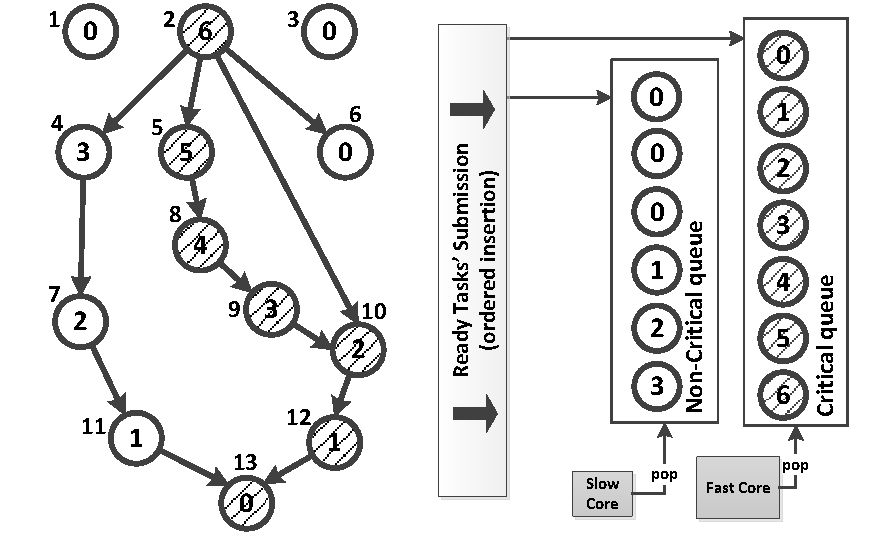
\includegraphics[width=\columnwidth]{images/fig_1.pdf} 
\centering
\caption{CATS overview. Nodes are marked with the \textit{bottom level} of each task. Pattern-filled nodes mark the critical tasks.}
\label{botlevels}
\vspace{-0.5cm}
\end{figure}


\subsection{Task Prioritization}

Each task in the TDG has a list to include its predecessors (\textit{plist}). Every time an edge is added into the TDG on the creation of a new task, the corresponding predecessor of the dependency is added in the \textit{plist} of its successor. For example, in Figure~\ref{botlevels}, when the dependency between tasks~2 and~5 occurs, the task number~2 is inserted into the \textit{plist} of the task number~5. Thus, the \textit{plist} of task number~5 becomes $\{$2$\}$. Accordingly, the \textit{plist} of task number~10 will be $\{$2, 9$\}$ when the edge~9$\rightarrow$10 is inserted to the TDG. 

%Right after the occurrence of a dependency between two tasks, the task prioritization step takes place, once for each edge of the graph. 
%represented by the edges in the graph, that connect one predecessor task with one successor task.

The priority given to a task is the \textit{bottom level} of the task. The \textit{bottom level} is computed by traversing the TDG upwards starting from the successor that the currently created edge is pointing to. The priority of this successor is 0 because it is a leaf node of the graph, as it is the last created task. Then, using \textit{plist} for each task, the algorithm navigates to the upper levels of the TDG and updates the priority on each visited node. This way not all the graph is updated, but only the tasks that are predecessors in the paths to the new edge. The algorithm also stops going up through a path, when it finds a priority larger than the one it would be updated to.

Listing~\ref{creation} shows the algorithm for task prioritization. The complexity of this is \textit{O($n^2$)}, \textit{$n$} being the number of tasks. This function is called on the creation of a new edge with the successor as argument. The algorithm traverses the \textit{plist} of the successor task (line 5) and if the priority of the current predecessor is lower than the bottom level of the successor plus one, it updates the current predecessor's priority to that value (lines 7-8). If the updated predecessor task is ready (i.e., it sits in one of the ready queues), the scheduler reorders the ready queue so it remains ordered considering the updated priority (lines 9-10). Then, the same actions are performed recursively for each predecessor of the \textit{plist} to update all the possible upward paths from the successor. 

The terminate conditions for the TDG navigation are two: \textit{(a)} if the \textit{plist} of the current task (\texttt{currPred}) is empty, so either we reach an entry node or the predecessors of the task have finished execution; or \textit{(b)} if the priority of the current task (\texttt{currPred}) remains unchanged, which means that the successor task (\texttt{succ}) does not belong to the longest path because its predecessor already has a higher priority. 
\begin{lstlisting}[float, emph={void,if,return,non_critical_queue, critical_queue,prioritize_task}, captionpos=b, caption={Pseudo-code task prioritization with CATS.},label=creation, emph={[2]mat}, emphstyle={[2]}, aboveskip={0\baselineskip}, frame=tb, belowskip={-0.4cm}]
1 void prioritize_task(task *succ) {
2  int blev = succ->priority;
3  list plist = plistOf(succ);
4  task *currPred;
5  while( not isEmpty(plist) ) {
6    currPred = plist.next();  
7    if(priorityOf(currPred) < blev+1) {
8     currPred->priority = blev+1;
9     if(isReady(currPred)) 
10     readyQueueOf(currPred)->reorder();
11    prioritize_task(currPred);
12   }
13 }
14}
\end{lstlisting}
\subsection{Task Submission}

%CATS supports two task submission policies: the \textit{flexible} policy adds more task in the critical queue for the fast cores, while the \textit{strict} policy reduces the number of critical tasks.

The purpose of this step is to divide the tasks into two groups: \textit{critical} and \textit{non-critical}. Critical tasks are tasks that belong to the longest path of the dynamic TDG, namely the path  with the maximum number of tasks (or nodes). Thus, the longest path starts from the task with the maximum bottom level. At runtime, the longest path changes as tasks complete execution and new tasks are created. CATS manages to detect these changes and dynamically decide if the submitted task belongs to the longest path of the TDG.

When a task's dependencies are satisfied, the task becomes ready for execution and is to be inserted in the \textit{ready queues}. Ready queues are priority queues that keep tasks in a decreasing order of task priorities, i.e., the task with the maximum priority resides on the head of the queue. Critical tasks are inserted in the critical queue and non-critical tasks in the non-critical queue. The pattern-filled nodes in Figure~\ref{botlevels} represent the critical tasks in that graph. 

%This way, tasks in the critical queue will then be scheduled to fast cores, and non-critical tasks to slow cores.

%By keeping track of the last discovered critical task%task with the maximum priority
To determine the criticality of a task, CATS keeps track of the last discovered critical task. Then, for each task that becomes ready, CATS checks the following conditions:
%, our approach to detect critical tasks in the graph is to check the following two conditions for each task that becomes ready:
\textit{(a)} if the priority of the current ready task is higher or equal to the priority of the last discovered critical task and, \textit{(b)} if the current ready task is the highest-priority immediate successor of the last discovered critical task.

%%%%%%%%%%%%%%%%%%%%%%%%%%%%%%%%%%%%%%%%
%flexible strict explanation
In the first case, the algorithm detects new longest paths that may have been created by the application throughout the execution of a prior longest path. In this case, the scheduler can either be \textit{strict} or \textit{flexible}:
\begin{itemize}
 \item{\textit{Strict}: marks as critical tasks with priority higher than the priority of the last critical task.}
 \item{\textit{Flexible}: marks as critical tasks with priority higher or equal to the priority of the last critical task.} 
 \end{itemize}
As a result, the flexible scheduler ends up with more critical tasks than the strict. The flexibility of the scheduler can be set by the programmer through an environment variable.
% about flexible/strict explanation
%%%%%%%%%%%%%%%%%%%%%%%%%%%%%%%%%%%%%%%%%%%%
\begin{figure}[tl!]
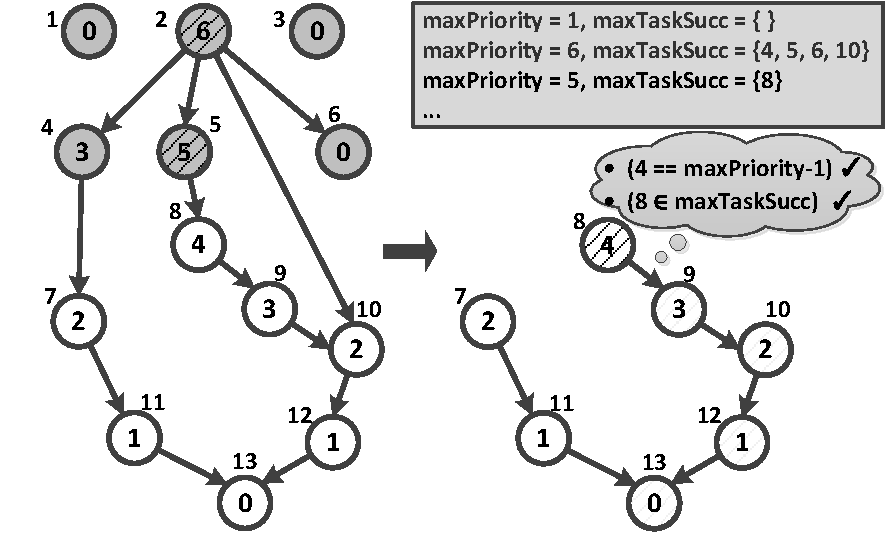
\includegraphics[width=\columnwidth]{images/fig_2.pdf} 
\centering
\caption{Task submission with CATS. Gray nodes indicate finished tasks and pattern-filled nodes indicate critical tasks.}
\label{submitFig}
\vspace{-0.5cm}
\end{figure}
The task that satisfies the second condition is a task with a lower priority than the maximum but the task belongs to the longest path because it is the highest priority immediate successor of the last detected critical task. 

Listing~\ref{submission} shows a simplified version of the task submission code, that is of complexity \textit{O($n$)} (\textit{$n$} is the number of tasks). The variable \texttt{maxPriority} (line 1) is used to store the priority of the last critical task, and \texttt{maxPriorityTask} (line 2) is used to store the last critical task. Initially, \texttt{maxPriority} is set to 1 and \texttt{maxPriorityTask} is set to \texttt{NULL}. This avoids the scheduling of independent tasks (i.e., tasks with zero priority) to fast processors at the start of the execution. On the first ready task, if its priority is higher or equal than 1 (line 5) , it is considered to be the first task of the longest path. Therefore, it is inserted in the critical queue and the variables \texttt{maxPriority} and \texttt{maxPriorityTask} are updated accordingly (lines 9-11) to determine correctly the criticality of the next submitted task.

If the priority of the submitted task is equal to \texttt{maxPriority - 1}, we check if it also belongs to the successors of the task with the maximum priority (lines 6-7) and therefore to the longest path. If these two conditions are met, the task is determined to be critical, it is inserted in the critical queue and, as before, the variables \texttt{maxPriority} and \texttt{maxPriorityTask} are updated (lines 9-11). In the rest of the cases the task is not considered critical and it is inserted in the non-critical queue.

Figure~\ref{submitFig} shows an example of a TDG during task submission. The gray nodes in the graph are tasks that have finished execution and the pattern-filled nodes are critical tasks. The numbers inside the nodes indicate their priority and the numbers outside the nodes show the task id, which is assigned in task creation order. The variable \texttt{maxPriority} corresponds to the priority of the last critical task and the \texttt{maxTaskSucc} is the list of the successors of the last critical task, filled with the task ids of the successors. Initially, \texttt{maxPriority} is set to~1 and \texttt{maxTaskSucc} is empty. When task~2 is about to be submitted, it is inserted in the critical queue because its priority is higher than the maximum, which at the beginning is~1. Then, the value of \texttt{maxPriority} is set to~6 (priority of task~2), and the \texttt{maxTaskSucc} list is updated with the successors of task~2. At the point where all the gray tasks have finished execution, the values of \texttt{maxPriority} and \texttt{maxTaskSucc} are updated as shown  in Figure~\ref{submitFig}. For every newly-ready task, the conditions listed above are evaluated. When task~7 is submitted, it is not considered as critical because it does not belong to the \texttt{maxTaskSucc} list and its priority is not equal to \texttt{maxPriority-1}. Contrarily, task 8 satisfies both conditions and so the task is inserted in the critical queue.

\begin{lstlisting}[float, emph={void,if,return,non_critical_queue, critical_queue,submit_task}, captionpos=b, caption={Pseudo-code for task submission with CATS.},label=submission, emph={[2]mat}, emphstyle={[2]}, aboveskip={0\baselineskip}, frame=tb, belowskip={-0.4cm}]
1 int maxPriority = 1;
2 task *maxPriorityTask = NULL;
3
4 void submit_task(task *t) {
5  if( t->priority >= maxPriority or
6     (t->priority == maxPriority-1 and
7      t $\in$ succListOf(maxPriorityTask)) )
8  { //the task is critical
9    critical_queue.push(t);
10   maxPriority = priorityOf(t);
11   maxPriorityTask = t;
12   return;
13 }
14 //the task is non-critical
15 non_critical_queue.push(t);     
16}
\end{lstlisting}

\subsection{Task-to-Core Assignment}
\label{sec.cats.assignment}
Task-to-core assignment takes place dynamically and in parallel to the previous steps and its time complexity is \textit{O($n$)}, \textit{$n$} being the number of tasks. When a core becomes idle, it checks the corresponding ready queue (depending on the core type) to get a task to execute. Fast cores retrieve critical tasks from the critical queue, while slow cores retrieve non-critical tasks from the non-critical queue. Each ready queue is shared among the cores of the same type so there is no need for work stealing among cores of the same type. 

If tasks in an application are imbalanced, i.e., the majority are non-critical and only a few tasks are critical, or vice versa, one of the types of processors would be overloaded and the other would starve for work. This can happen in applications with wide graphs and a large amount of tasks, where the ratio between critical tasks and the total amount of tasks may be small. To leverage the resources, the work-stealing mechanism for CATS lets fast cores steal work from slow cores whenever the critical queue becomes empty. 
Also, CATS can be configured to perform \textit{bidirectional work stealing} so slow processors can also steal tasks from the critical queue if the non-critical queue is empty. 
We evaluate these different options and show the results in Section~\ref{sec.cats_eval}.
